\documentclass[11pt]{article}
\usepackage[margin=1in]{geometry}
\usepackage[T1]{fontenc}
\usepackage{mathptmx,amsmath,booktabs,threeparttable,graphicx,placeins,natbib}
\usepackage[font=small,labelfont=bf]{caption}
\usepackage[colorlinks=true,allcolors=blue]{hyperref}
\setlength{\emergencystretch}{2em}
\title{Measuring the Right to Know:\\Early Evidence from an Online RTI Audit in India}
\author{Priyadarshi Amar \and Gaurav Sood}
\date{Working draft: data through 29 October 2026}
\pdftrailerid{}
\begin{document}
\maketitle
\begin{abstract}
A recorded response to an information request need not provide information. We study this distinction using standardized requests for public authorities' own Right to Information (RTI) records in Tamil Nadu, Telangana, Karnataka, Delhi, and Maharashtra. Of 1,665 drawn applications, 996 had been filed by the data cutoff and 455 had reached thirty days. Excluding Telangana, where portal outcomes are especially poorly observed, 28.7 percent of these mature applications had a recorded response within thirty days, while 14.2 percent had documented provision of information. These are interim, sample-conditional rates; incomplete retrieval also affects the other jurisdictions. A randomized legal-salience paragraph produces imprecise estimates, with no basis for concluding that reminders have no effect. The results distinguish administrative activity from substantive disclosure and identify the observation and sampling conditions needed for a broader assessment of the RTI regime.
\end{abstract}

\section{Introduction}
The operation of a right to information depends on what a citizen receives after asking. A portal can register an application, mark it disposed, or forward it without supplying the requested records. Measuring these steps separately matters for assessing access: a recorded administrative action and an answer to the question serve different purposes.

We examine requests for each public authority's own RTI register and reporting records. This common subject makes offices more comparable than a collection of unrelated requests, while locating the inquiry in the administration of the transparency regime itself. The requests ask for existing records, permit alternative levels of aggregation, and do not ask for applicants' names or addresses. The design document in the companion \texttt{in-rolls/rti} repository motivates a descriptive audit with embedded randomized variation. This paper implements that framework on the existing frozen snapshot; it does not report the completion of the larger proposed study.

The observed gap between response and information is substantial. Among mature applications outside Telangana, the recorded response rate is 28.7 percent and the information-supplied rate is 14.2 percent. Neither number establishes the true rate of silence: some answers remain on portals or in postal channels outside the retrieved record. The distinction is therefore between observed activity and documented information receipt. It is not an estimate of unlawful refusal.

The study connects two strands of research. \citet{peisakhin} show that an RTI application can help applicants obtain ration cards in Delhi. Their outcome is access to a service; ours is access to the requested information. \citet{worthy} compare statutory and informal requests to English parish councils. Our contrast is narrower: both arms use the statutory channel, and one adds a reminder of deadlines and penalties. Finally, \citet{berliner} study the topics of information requests in Mexico. The registers requested here could eventually support an analogous account of demand, but only conditional on obtaining those records. This interim paper concerns the response to the register request itself.

\section{Design and scope}
\subsection{The request and the sampling frame}
The instrument requests the authority's RTI record for the preceding twelve months and its Section 25 return. Acceptable responses include application-level records, category counts, or period totals. Full disclosure requires register information and either the return or a statement that the return is not held. Partial disclosure requires some requested information actually present in the retrieved material. This operational definition measures content supplied, rather than a letter's assertion that an enclosure was sent.

Offices were drawn from portal authority rosters. Tamil Nadu uses department-by-tier quotas, with separate department, head-of-department, and sub-office categories. Telangana and Karnataka use department-group sampling with caps; Delhi and Maharashtra also use department-group sampling. These are different designs, and their pooled realized sample is not a probability sample of all Indian public authorities. The analysis preserves their distinct treatment blocks rather than treating administrative departments as interchangeable randomization strata.

The intended population in the local design document is the set of offices reachable through online portals. The present analytic population is narrower still: drawn offices whose applications were successfully filed and had sufficient follow-up by the cutoff. Table~\ref{tab:tab_sample} documents this transition. Filing order was not randomized. Differences between the drawn and mature samples can therefore change both the descriptive population and the interpretation of treatment comparisons.
\begin{table}[!htbp]
\centering
\caption{Sample and filing by state}
\label{tab:tab_sample}
\small
\begin{threeparttable}
\begin{tabular}{lrrrrrrl}
\toprule
State & Frame & Drawn & Plain / legal & Filed & Filed (\%) & Past day 30 & Filing window \\
\midrule
Tamil Nadu & 17,417 & 1,000 & 700 / 300 & 528 & 52.8 & 140 & 26 Aug to 28 Oct \\
Telangana & 3,401 & 375 & 262 / 113 & 218 & 58.1 & 187 & 04 Sep to 24 Oct \\
Karnataka & 1,800 & 180 & 126 / 54 & 149 & 82.8 & 78 & 11 Sep to 28 Oct \\
Delhi & 223 & 44 & 30 / 14 & 44 & 100.0 & 22 & 19 Sep to 26 Oct \\
Maharashtra & 328 & 66 & 46 / 20 & 61 & 92.4 & 28 & 15 Sep to 27 Oct \\
\midrule
All & 23,169 & 1,665 & 1,164 / 501 & 1,000 & 60.1 & 455 & 26 Aug to 28 Oct \\
\bottomrule
\end{tabular}
\begin{tablenotes}[flushleft]\footnotesize
\item \textit{Notes:} Data as of 29 October 2026. Past day 30: filed by 29 September, so the 30-day limit in s.7(1) has passed. Tamil Nadu is drawn by department $\times$ tier quotas, other states proportionally to department group with a cap.
\end{tablenotes}
\end{threeparttable}
\end{table}

\FloatBarrier

\subsection{Legal salience and applicant characteristics}
The legal-salience letter adds a reference to the Section 7(1) deadline and Section 20 penalties. The plain letter omits that paragraph. Maharashtra uses a shorter instrument because of its portal's word limit, so the appendix reports a specification excluding it. The contrast does not isolate a particular psychological mechanism: the reminder could convey awareness of the law, willingness to follow up, or an expectation of enforcement.

Tamil Nadu assigns treatment within department-by-tier strata. Telangana and Karnataka assign it over the batch, while Delhi and Maharashtra assign it within state and batch. The analysis uses department-by-tier blocks for Tamil Nadu and state-by-batch blocks elsewhere. Department-group controls in the latter states are additional adjustments, not a description of the assignment mechanism.

The design does not manipulate applicant identity. Research-assistant labels do not identify independent people: some labels refer to the same filer. Phone reachability is bundled with filer name and postal address. Consequently, filer and phone comparisons are descriptive and cannot identify gender, identity, or telephone-access effects.

\section{Data and measurement}
The frozen dataset joins assignment lists, filing sheets, email events, and coded reply documents. Assignment files are pinned to upstream commits and checksums. Filing requires a real registration number or a portal acknowledgment; free text in the registration-number field is insufficient. The derived data contain one row per drawn application. Repeat submissions to an office remain part of that application's history rather than becoming new randomized units.

The snapshot contains 996 filed applications out of 1,665 drawn, with 455 observed for at least thirty days. Reply dates use the letter date where legible and otherwise the recorded arrival date, so elapsed time is not uniformly time to applicant receipt. The outcome window starts from the recorded filing date, using the portal date where available and otherwise the filing sheet. A common thirty-day window permits comparison, but does not adjudicate each case's legal deadline: transfers, fee requests, or other procedures can change the applicable clock.

We distinguish three nested outcomes. Any response includes a recorded office action, including a transfer or fee demand. Reply excludes transfers but includes fee demands. Information supplied requires a reply coded full or partial. Phone calls are reported separately. Applications with insufficient exposure do not enter fixed-horizon denominators. Survival curves use their available follow-up, with administrative censoring at the cutoff.

Outcome observation differs across portals. Telangana's portal supplies filing acknowledgments without corresponding status emails, and the frozen filing sheets do not record status checks. Delhi and Maharashtra also lack status notices in the inboxes. Missing downloads and unlogged postal arrivals further limit ascertainment. A zero in a recorded-response indicator therefore need not mean that an office did nothing. Even the sample excluding Telangana does not eliminate this problem.

The reply corpus contains 104 coded replies, of which 54 supply some information and 15 meet the full-disclosure definition. These corpus totals include replies outside the thirty-day analysis window and must not be used as its numerator. The first coding pass, second pass, and adjudication were conducted with Claude in separate contexts. Agreement on information supplied is 92 percent; agreement on disposition is 74 percent. Agreement between model runs is not validation against human judgment. Human review and access to the underlying documents are needed before treating the coding as a validated measure of substantive compliance.

\section{Analysis}
For each jurisdiction, the principal descriptive statistic is the proportion of mature filed applications with a recorded event by day thirty. These rates pool both letter arms and describe the realized intervention mixture. They are not estimates of the plain-letter baseline proposed in the design document. Table~\ref{tab:tab_main} separately reports the plain-letter mean within each regression sample.

The Tamil Nadu standardization weights tier-specific mature-sample rates by the tier shares in the portal frame. It illustrates sensitivity to the sample's tier composition; it does not recover department inclusion probabilities or adjust for selective filing and follow-up. Its interpretation requires transportability of the early tier-specific rates to the wider frame, which the current data do not establish.

Treatment comparisons use linear probability models with the appropriate block fixed effects and heteroskedasticity-robust standard errors. Outcomes are scaled to percentages, so coefficients are percentage-point differences. Tamil Nadu is estimated separately. The appendix preserves alternative department-group adjustments, later horizons, and exploratory survival models. Randomization-inference results condition on the analyzed sample and observed treatment totals within blocks; specifications with department-group fixed effects further condition on block-by-department-group treatment totals. These conditional tests do not remove selection into that sample.

Conditioning on filing and maturity occurs after treatment assignment. A causal reading consequently requires that assignment did not affect inclusion, and that outcome ascertainment is comparable across arms. Balance diagnostics and filing rates can reveal problems but cannot establish those assumptions. The estimates below are interim comparisons from an ongoing experiment, not confirmatory tests certified by a prospective registration.

\section{Results}
\subsection{Recorded response and information receipt}
Table~\ref{tab:tab_response_state} reports observed outcomes. Tamil Nadu records a response within thirty days for 12.9 percent of mature applications; Karnataka records 52.6 percent. Telangana's 1.1 percent should be read as a recorded lower bound, given its missing portal monitoring. Cross-state differences combine office composition, filing schedules, and observation systems with any underlying differences in responsiveness. They do not identify the effect of a state administration.

Outside Telangana, 28.7 percent have any recorded response and 14.2 percent have documented information. A transfer can move an application toward the appropriate custodian, and a fee demand can precede eventual disclosure. Both register activity without establishing that information has reached the applicant. Conversely, a disposal notice without its document leaves substantive provision unknown. Reporting each stage avoids treating these different processes as equivalent success.
\begin{table}[!htbp]
\centering
\caption{Response within 30 days of filing, by state (\%)}
\label{tab:tab_response_state}
\small
\begin{threeparttable}
\begin{tabular}{lrrcrr}
\toprule
State & N & Any response & 95\% CI & Reply & Information supplied \\
\midrule
Tamil Nadu & 140 & 12.9 & [8.3, 19.4] & 12.1 & 5.0 \\
\quad tier-standardized &  & 7.0 & [2.6, 11.4] & 6.9 & 2.1 \\
Telangana & 187 & 1.1 & [0.3, 3.8] & 1.1 & 1.1 \\
Karnataka & 78 & 52.6 & [41.6, 63.3] & 51.3 & 28.2 \\
Delhi & 22 & 22.7 & [10.1, 43.4] & 18.2 & 13.6 \\
Maharashtra & 28 & 46.4 & [29.5, 64.2] & 35.7 & 21.4 \\
\midrule
All states & 455 & 17.4 & [14.2, 21.1] & 16.0 & 8.8 \\
All excl. Telangana & 268 & 28.7 & [23.6, 34.4] & 26.5 & 14.2 \\
\bottomrule
\end{tabular}
\begin{tablenotes}[flushleft]\footnotesize
\item \textit{Notes:} Applications past day 30. Any response: any office action, including a transfer or fee demand. Reply: excludes transfers. Information supplied: reply coded full or partial, a lower bound. Telangana is a lower bound because its portal sends no status emails. Intervals: 95\% Wilson, except normal for the tier-standardized row.
\end{tablenotes}
\end{threeparttable}
\end{table}

\FloatBarrier

Tamil Nadu's tier-standardized response rate is 7.0 percent, below its unweighted rate. This difference demonstrates the importance of the office mix. It does not resolve the remaining selection of departments and filing dates. The survival curves in Figure~\ref{fig:fig_km_state} describe the timing of recorded events among filed applications. Their censoring adjustment requires assumptions about follow-up and observation that can fail when filing sequence tracks office characteristics; they do not recover unobserved portal replies.
\begin{figure}[!htbp]
\centering
\caption{Time to first response, by state}
\label{fig:fig_km_state}
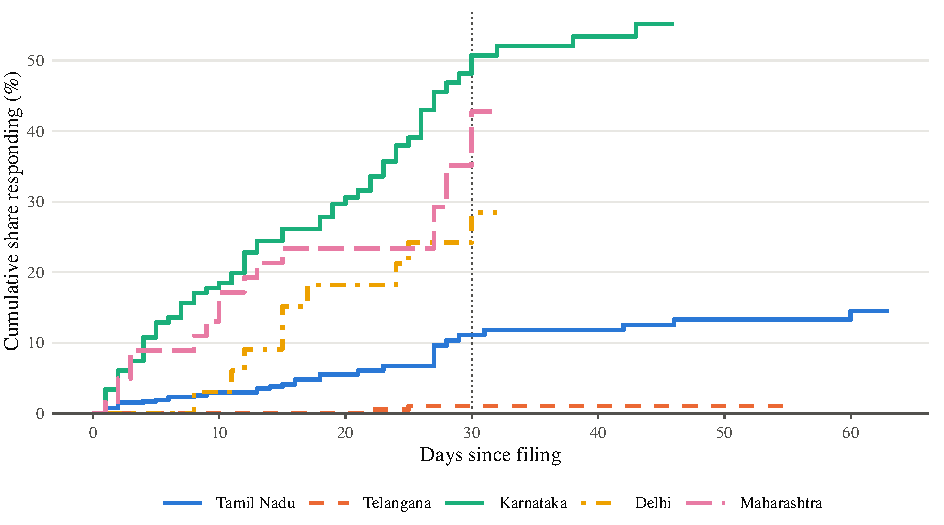
\includegraphics[width=\textwidth]{figures/fig_km_state.pdf}
\begin{minipage}{\textwidth}\footnotesize
\textit{Notes:} Kaplan-Meier estimates of time to any response (any office action, including a transfer or fee demand), all 999 dated filings, censored at 29 October; curves stop when fewer than 10 applications remain at risk. Dotted line: the 30-day limit in s.7(1). Telangana is a lower bound because its portal sends no status emails.
\end{minipage}
\end{figure}

\FloatBarrier

\subsection{Legal-salience comparisons}
The block-adjusted difference in any recorded response is 1.1 percentage points in Tamil Nadu (standard error 5.8) and 3.6 points in the other states (standard error 3.9). Excluding Telangana from the latter group yields 10.9 points (standard error 9.3). Table~\ref{tab:tab_main} reports the other outcomes and alternative adjustments. These specifications address different realized samples, and their differences should not be presented as independent replications.

The estimates are too imprecise to establish that legal reminders are ineffective. The table's detectable-effect heuristic, calculated as a multiple of the estimated standard error, is an interim precision diagnostic rather than prospective power for the original design. Department-group fixed effects also change the observations retained and leave limited within-group treatment variation. A large coefficient in that specification is not stronger evidence merely because it is larger.
\begin{table}[!htbp]
\centering
\caption{Effect of the legal-salience letter}
\label{tab:tab_main}
\small
\begin{threeparttable}
\begin{tabular}{lrrrrrr}
\toprule
& \multicolumn{2}{c}{Tamil Nadu} & \multicolumn{2}{c}{Other states} & \multicolumn{2}{c}{Excl. Telangana} \\ \cmidrule(lr){2-3}\cmidrule(lr){4-5}\cmidrule(lr){6-7}  & (1) & (2) & (3) & (4) & (5) & (6) \\
\midrule
\addlinespace\multicolumn{7}{l}{\textit{Panel A. Any response by day 30}} \\
Legal letter & $-$0.1 & 1.1 & 2.6 & 7.0 & 8.5 & 31.3 \\
 & (6.0) & (5.8) & (3.9) & (3.8) & (9.4) & (13.5) \\
Plain-letter mean & 12.9 & 9.1 & 18.0 & 12.0 & 42.5 & 39.1 \\
Detectable effect (2.8 $\times$ SE) & 16.9 & 16.2 & 10.9 & 10.6 & 26.3 & 37.8 \\
Randomization-inference $p$ &  & 1.000 & 0.569 & 0.144 & 0.440 & 0.069 \\
N & 140 & 128 & 315 & 242 & 128 & 73 \\
\addlinespace\multicolumn{7}{l}{\textit{Panel B. Reply by day 30}} \\
Legal letter & 2.0 & 2.3 & 2.8 & 6.3 & 8.9 & 28.3 \\
 & (5.9) & (5.6) & (3.9) & (3.6) & (9.2) & (13.0) \\
Plain-letter mean & 10.8 & 8.0 & 15.7 & 10.8 & 36.8 & 34.8 \\
Detectable effect (2.8 $\times$ SE) & 16.4 & 15.7 & 10.8 & 10.1 & 25.9 & 36.4 \\
Randomization-inference $p$ &  & 0.703 & 0.551 & 0.174 & 0.415 & 0.125 \\
N & 140 & 128 & 315 & 242 & 128 & 73 \\
\addlinespace\multicolumn{7}{l}{\textit{Panel C. Information supplied by day 30}} \\
Legal letter & 0.0 & $-$0.6 & $-$3.5 & $-$0.9 & $-$6.2 & 0.5 \\
 & (3.6) & (3.4) & (3.1) & (2.9) & (7.5) & (10.8) \\
Plain-letter mean & 4.3 & 3.4 & 10.1 & 7.2 & 23.0 & 21.7 \\
Detectable effect (2.8 $\times$ SE) & 10.2 & 9.5 & 8.8 & 8.0 & 21.0 & 30.3 \\
Randomization-inference $p$ &  & 1.000 & 0.366 & 1.000 & 0.486 & 1.000 \\
N & 140 & 128 & 315 & 242 & 128 & 73 \\
\midrule
Randomization-block FE & No & Yes & Yes & Yes & Yes & Yes \\
Department-group FE & No & No & No & Yes & No & Yes \\
\bottomrule
\end{tabular}
\begin{tablenotes}[flushleft]\footnotesize
\item \textit{Notes:} Linear probability models, applications past day 30, percentage points, robust SEs. Legal letter: cites the s.7(1) deadline and s.20 penalties. Any response includes transfers and fee demands; reply excludes them; information: coded full or partial. Blocks: department $\times$ tier (Tamil Nadu), state $\times$ batch (others). Columns (4), (6) rest on 162, 41 applications in department groups with both letters.
\end{tablenotes}
\end{threeparttable}
\end{table}

\FloatBarrier

\section{Discussion}
The existing evidence supports a distinction between recorded administrative action and documented disclosure. It does not yet support a national compliance rate, a causal ranking of states, or a definitive estimate of the legal-salience effect. Those boundaries follow from the data-generating process: the mature sample is selected from an unfinished filing program, portal observation varies, and substantive coding has not received human validation.

The local design document asks broader questions about demand composition, exemption use, appeals, and discrepancies between office-reported and applicant-observed performance. The current tables do not answer those questions. Register-based analyses would condition on obtaining a register, while an office-level discrepancy requires comparable reporting periods and definitions on both sides. Longer follow-up is also needed for the proposed later horizons and appeals. Neither the absence of these analyses nor an early null should be turned into evidence about their eventual outcomes.

Before a submission-ready version, the most valuable work is to retrieve outstanding portal and postal responses, validate content coding against documents, and document selection from assignment through filing and follow-up. Those tasks improve measurement directly. Additional regression specifications cannot substitute for them. The present draft preserves the frozen evidence so that later data collection can be distinguished from retrospective analytical changes.

\begin{thebibliography}{9}
\bibitem[Peisakhin and Pinto(2010)]{peisakhin} Peisakhin, Leonid, and Paul Pinto. 2010. Is transparency an effective anti-corruption strategy? Evidence from a field experiment in India. \emph{Regulation \& Governance} 4:261--280. \href{https://doi.org/10.1111/j.1748-5991.2010.01081.x}{doi:10.1111/j.1748-5991.2010.01081.x}.
\bibitem[Worthy et al.(2017)]{worthy} Worthy, Ben, Peter John, and Matia Vannoni. 2017. Transparency at the Parish Pump: A Field Experiment to Measure the Effectiveness of Freedom of Information Requests in England. \emph{Journal of Public Administration Research and Theory} 27:485--500. \href{https://doi.org/10.1093/jopart/muw063}{doi:10.1093/jopart/muw063}.
\bibitem[Berliner et al.(2018)]{berliner} Berliner, Daniel, Benjamin E. Bagozzi, and Brian Palmer-Rubin. 2018. What Information Do Citizens Want? Evidence from One Million Information Requests in Mexico. \emph{World Development}. \href{https://doi.org/10.1016/j.worlddev.2018.04.016}{doi:10.1016/j.worlddev.2018.04.016}.
\end{thebibliography}

\clearpage
\appendix
\section{Design provenance and departures}
The reference design is \texttt{ms/ms.tex} in \texttt{in-rolls/rti}, at commit \texttt{a2815a4}. The existing analysis documentation refers to an Overleaf \texttt{main.tex}; equivalence to that unavailable file has not been established. The manuscript uses the local document specified by the authors. No registration record was supplied, so the design's prospective language is not evidence that this interim analysis was registered.

The reference design places primary descriptive weight on the plain arm and specifies broader geography and later follow-up. This snapshot pools arms for the state summaries, uses the existing jurisdictions, and emphasizes the thirty-day window. The Cox specifications and permutation tests are additions documented by the upstream analysis. Tier standardization is confined to Tamil Nadu. Peer-information treatments, the reservation-records arm, appeals, and commission-report comparisons are outside this analysis. These distinctions are retained as departures rather than silently rewriting the design around available outcomes.

\section{Additional exhibits}
Table~\ref{tab:tab_balance} reports filing and maturity by arm among drawn applications and the treatment composition of Tamil Nadu tiers; Table~\ref{tab:tab_content} separates the content of retrieved replies. Table~\ref{tab:tab_robust} compares alternative horizons and specifications, whose eligible samples differ. These checks describe sensitivity within the observed data and cannot correct missing portal outcomes or establish human coding validity.
\begin{table}[!htbp]
\centering
\caption{Does the letter predict who is filed and who has reached day 30?}
\label{tab:tab_balance}
\small
\begin{threeparttable}
\begin{tabular}{lrrrrrrr}
\toprule
& & \multicolumn{3}{c}{Filed (\%)} & \multicolumn{3}{c}{Past day 30 (\%)} \\ \cmidrule(lr){3-5}\cmidrule(lr){6-8} State & N & Plain & Legal & $p$ & Plain & Legal & $p$ \\
\midrule
\addlinespace\multicolumn{8}{l}{\textit{Panel A. All drawn applications}} \\
Tamil Nadu & 1,000 & 52.0 & 53.7 & 0.867 & 13.3 & 15.7 & 0.901 \\
Telangana & 375 & 57.6 & 59.3 & 0.702 & 49.6 & 50.4 & 0.774 \\
Karnataka & 180 & 81.7 & 83.3 & 0.797 & 41.3 & 48.1 & 0.399 \\
Delhi & 44 & 100.0 & 100.0 &  & 50.0 & 50.0 &  \\
Maharashtra & 66 & 93.5 & 90.0 & 0.641 & 43.5 & 40.0 & 0.641 \\
\midrule
\addlinespace\multicolumn{8}{l}{\textit{Panel B. Tamil Nadu past day 30, by tier}} \\
 & N & Plain & Legal &  & Legal (\%) & Drawn (\%) &  \\
Department & 7 & 0 & 7 &  & 100.0 & 32.5 &  \\
Head of Department & 21 & 15 & 6 &  & 28.6 & 25.7 &  \\
Sub Office & 112 & 78 & 34 &  & 30.4 & 30.6 &  \\
\bottomrule
\end{tabular}
\begin{tablenotes}[flushleft]\footnotesize
\item \textit{Notes:} Past day 30: filed by 29 September. Panel A: $p$-values on the letter in a linear probability model with randomization-block fixed effects and robust SEs. Panel B: counts, with the legal share among them and among all drawn in that tier. All 7 department-tier filings past day 30 got the legal letter.
\end{tablenotes}
\end{threeparttable}
\end{table}

\FloatBarrier
\begin{table}[!htbp]
\centering
\caption{What the coded replies contain}
\label{tab:tab_content}
\small
\begin{threeparttable}
\begin{tabular}{lrrrr}
\toprule
 & Tamil Nadu (26) & Others (78) & All (104) & All (\%) \\
\midrule
\addlinespace\multicolumn{5}{l}{\textit{Disposition}} \\
\quad Full information & 4 & 23 & 27 & 26 \\
\quad Partial information & 4 & 16 & 20 & 19 \\
\quad Fee asked first & 6 & 12 & 18 & 17 \\
\quad Denied or deflected & 6 & 4 & 10 & 10 \\
\quad Returned & 1 & 15 & 16 & 15 \\
\quad Transferred & 5 & 8 & 13 & 12 \\
\addlinespace\multicolumn{5}{l}{\textit{Data supplied}} \\
\quad Application-level register & 5 & 21 & 26 & 25 \\
\quad Monthly or category counts & 1 & 5 & 6 & 6 \\
\quad Period totals & 4 & 11 & 15 & 14 \\
\quad Prose only & 0 & 2 & 2 & 2 \\
\quad None & 16 & 39 & 55 & 53 \\
\addlinespace\multicolumn{5}{l}{\textit{Section 25 annual return}} \\
\quad Supplied & 3 & 15 & 18 & 17 \\
\quad Not held & 3 & 3 & 6 & 6 \\
\quad Offered on payment & 5 & 4 & 9 & 9 \\
\quad Told to apply separately & 0 & 2 & 2 & 2 \\
\quad Referred to website & 1 & 1 & 2 & 2 \\
\quad Not addressed & 14 & 53 & 67 & 64 \\
\addlinespace\multicolumn{5}{l}{\textit{How it arrived}} \\
\quad Post & 17 & 34 & 51 & 49 \\
\quad Portal & 8 & 26 & 34 & 33 \\
\quad Email & 1 & 18 & 19 & 18 \\
\addlinespace\multicolumn{5}{l}{\textit{Provisions cited}} \\
\quad Exemption, s.8 & 0 & 2 & 2 & 2 \\
\quad Sections 2(f) or 7(9) & 6 & 4 & 10 & 10 \\
\quad Transfer, s.6(3) & 0 & 7 & 7 & 7 \\
\quad None & 19 & 64 & 83 & 80 \\
\bottomrule
\end{tabular}
\begin{tablenotes}[flushleft]\footnotesize
\item \textit{Notes:} All 104 coded replies, whenever they came. First-pass coding, not yet double-coded. Fees were quoted in 15 replies (median Rs 40, maximum Rs 832).
\end{tablenotes}
\end{threeparttable}
\end{table}

\FloatBarrier
\begin{table}[!htbp]
\centering
\caption{Legal-salience letter: alternative specifications}
\label{tab:tab_robust}
\footnotesize
\begin{threeparttable}
\begin{tabular}{lrrrrrr}
\toprule
& \multicolumn{2}{c}{Tamil Nadu} & \multicolumn{2}{c}{Other states} & \multicolumn{2}{c}{Excl. Telangana} \\ \cmidrule(lr){2-3}\cmidrule(lr){4-5}\cmidrule(lr){6-7}  & Coef. (SE) & N & Coef. (SE) & N & Coef. (SE) & N \\
\midrule
\addlinespace\multicolumn{7}{l}{\textit{Linear probability, any response (percentage points)}} \\
Baseline, by day 30 & 1.1 (5.8) & 128 & 2.6 (3.9) & 315 & 8.5 (9.4) & 128 \\
By day 35 & $-$0.1 (5.9) & 128 & 3.2 (3.7) & 269 & 13.3 (11.5) & 82 \\
By day 45 & 2.3 (5.6) & 128 & 3.5 (4.0) & 178 & 14.3 (16.5) & 40 \\
By day 14, all exposed that long & $-$0.5 (1.6) & 323 & 3.4 (3.4) & 393 & 6.5 (6.5) & 206 \\
Adding RA fixed effects & 1.2 (5.8) & 128 & 2.8 (3.9) & 315 & 8.9 (9.5) & 128 \\
Adding filing-week fixed effects & 1.3 (5.8) & 128 & 3.1 (3.9) & 315 & 11.1 (9.3) & 128 \\
Excluding Maharashtra (shorter letter) &  &  & 2.4 (3.8) & 287 & 9.4 (10.4) & 100 \\
RA2 and RA4 filings only & 4.3 (8.6) & 57 & $-$1.2 (6.6) & 140 & $-$2.3 (12.4) & 77 \\
RA1 and RA3 filings only & 3.1 (8.0) & 65 & 4.9 (4.7) & 175 & 21.3 (14.9) & 51 \\
\addlinespace\multicolumn{7}{l}{\textit{Cox model, all filings (hazard ratio)}} \\
Legal letter, stratified by block & 1.08 (0.45) & 527 & 1.40 (0.31) & 472 & 1.45 (0.32) & 254 \\
\bottomrule
\end{tabular}
\begin{tablenotes}[flushleft]\footnotesize
\item \textit{Notes:} All rows: any response (any office action, including a transfer or fee demand), legal letter as in Table~\ref{tab:tab_main}, block fixed effects, robust SEs. Later cutoffs and the day-14 row use applications exposed that long. Filer-group rows are exploratory. The Cox model is our addition, not in the design document; its SE is on the hazard-ratio scale.
\end{tablenotes}
\end{threeparttable}
\end{table}

\FloatBarrier

\section{Reproducibility and access}
The private analysis repository contains derived data, pinned upstream inputs, judgment-based coding files, and the scripts generating every exhibit and numerical statement. The manuscript template is filled from the same computed summaries used for the README. Running \texttt{make check} regenerates the analysis and both PDFs, then runs lint, tests, and privacy checks. Original emails, receipts, and reply documents remain outside Git because they contain personal information. Reproduction from the committed derived data does not independently validate their extraction. A raw-data rebuild requires the private archive matching the recorded manifest. No ethics approval or preregistration identifier is asserted in this draft; those records must be documented by the authors before submission.
\end{document}
